\documentclass[aoas,preprint]{imsart}

\usepackage[OT1]{fontenc}
\usepackage{amsmath}
\usepackage{natbib}
\usepackage[colorlinks,citecolor=blue,urlcolor=blue]{hyperref}
\usepackage{bm}
\usepackage{graphicx}

% settings
\pubyear{2016}
\volume{0}
\issue{0}
\firstpage{1}
\lastpage{23}

\startlocaldefs
\numberwithin{equation}{section}
\endlocaldefs
\bibliographystyle{imsart-nameyear}

\begin{document}

\begin{frontmatter}
\title{Efficient estimation of age-specific social contact rates between men and women}
\runtitle{Efficient estimation of social contact rates}

\begin{aug}
\author{\fnms{Jan} \snm{van de Kassteele}\thanksref{t1,m1}\ead[label=e1]{jan.van.de.kassteele@rivm.nl}},
\author{\fnms{Jan} \snm{van Eijkeren}\thanksref{m1}\ead[label=e2]{jan.van.eijkeren@rivm.nl}}
\and
\author{\fnms{Jacco} \snm{Wallinga}\thanksref{m2}\ead[label=e3]{jacco.wallinga@rivm.nl}}

\thankstext{t1}{Corresponding author}
\runauthor{J. van de Kassteele et al.}

\affiliation{Department of Statistics, Informatics and Mathematical Modeling. National Institute for Public Health and the Environment (RIVM)\thanksmark{m1} and Epidemiology and Surveillance Unit. National Institute for Public Health and the Environment (RIVM)\thanksmark{m2}}

\address{
Department of Statistics, Informatics\\
and Mathematical Modeling\\
National Institute for Public Health\\
and the Environment (RIVM)\\
PO Box 1, 3620BA\\
Bilthoven, the Netherlands\\
\printead{e1}\\
\phantom{E-mail:\ }\printead*{e2}}

\address{
Epidemiology and Surveillance Unit\\
National Institute for Public Health\\
and the Environment (RIVM)\\
PO Box 1, 3620BA\\
Bilthoven, the Netherlands\\
\printead{e3}}
\end{aug}

\begin{abstract}
Social contact patterns reveal with whom individuals tend to socialize, and therefore to whom they transmit respiratory infections. We infer highly detailed age-specific contact rates between the sexes using a hierarchical Bayesian model that smooths while simultaneously guarantees the inherent reciprocity of contact rates. Application of this approach to social contact data from a large prospective survey confirms a tendency that people, especially children and adolescents, mostly contact other people of their own age and sex, and reveals that women have more contact with children than men. These findings imply different exposure patterns between the two sexes for specific age groups, which agrees with available observations.
\end{abstract}

\begin{keyword}
\kwd{Social contact patterns}
\kwd{Hierarchical Bayesian model}
\kwd{Gaussian Markov Random Field}
\kwd{Integrated Nested Laplace Approximations}
\kwd{Infectious disease transmission}
\end{keyword}

\end{frontmatter}

\section{Introduction}

The incidence and severity of most human respiratory infections such as influenza, tuberculosis, measles, rubella, mumps, human parvovirus B19 and cytomegalovirus depend on age and sex \citep{falagas_sex_2007, klein_impact_2010, holmes_review_1998, borgdorff_gender_2000, neyrolles_sexual_2009, brown_sex_2010, davis_increasing_2010, young_parvovirus_2004, pass_vaccine_2009}. For the planning and evaluating of vaccination programs against these infectious diseases it is necessary to know how an infection spreads among age groups and among women and men. At-risk contacts for infection with respiratory pathogens are typically assessed via proxy measures, such as having a conversation or touching \citep{edmunds_who_1997, wallinga_using_2006, mossong_social_2008, kucharski_contribution_2014}. A quantitative understanding of the different contact behavior of men and women of various ages will thus contribute to a better understanding of how respiratory infections spread.

Even though sex differences in contact behavior have been a topic of general interest, there is surprisingly little scientific evidence to quantify the stereotypical gender roles of men and women \citep{mehl_are_2007}. \citet{mossong_social_2008} found no evidence of the daily number of social contacts being different for men and women when averaging over all ages. Further stratification by age revealed a strong tendency of girls contacting girls rather than boys, and vice versa in elementary schools \citep{cauchemez_role_2011, conlan_measuring_2011}. A recent study reported strong evidence of within-sex preferential mixing for broad age groups \citep{dodd_age-_2016}. However, to the best of our knowledge, there are no studies that offer precise estimates of the numbers of contacts by age and sex for a representative study population.

There is a large number of studies that collect data on at-risk contacts for infection using proxy measures such as having a conversation or touching \citep[e.g.]{edmunds_who_1997, wallinga_using_2006, mossong_social_2008, salathe_high-resolution_2010, read_close_2012, danon_social_2013, kucharski_contribution_2014, kwok_social_2014, eames_six_2015, dodd_age-_2016}; for textbooks that cover this field see \citet{vynnycky_introduction_2010, hens_modeling_2012}. Most of these studies follow the format of \citet{mossong_social_2008} and collect data on social contact behavior stratified by age and sex. These data have been used to infer contact rates that are relevant to the spread of a respiratory infection has been explored using mathematical modeling studies \citep[e.g.]{medlock_optimizing_2009, miller_incidence_2010, rohani_contact_2010, keeling_targeting_2011}. In all cases, the estimation has been limited to contact rates that are only age-specific, rather than age and sex specific. 

The estimation of contact rates by both age and sex from these data sets has proven to be statistically challenging for two reasons. First, the stratification by age and sex of both the study participants and their contacts leads to a very large number of contact rates (model parameters) to be estimated. For example, if we would choose to estimate the contacts by men and women in 81 age cohorts (age 0 - 80) to cover the age range in the general population, this would require estimating $(2 \times 81)^2 = 26,244$ contact rates. Second, the contact rates should also meet a reciprocity requirement. This requirement arises from the definition of a contact as a reciprocal event where two individuals have a conversation or touch. At the individual level, this implies that if John contacts Mary, Mary must have contacted John. Both issues, the need for regularization of the number of parameters while constraining to meet reciprocity, could result into computational problems.

There are relatively few statistical approaches to inferring contact rates from social contact data (see \citet{hens_modeling_2012}, ch. 15 for an overview). Most statistical analyses of social contact data, such as the one presented in \citet{mossong_social_2008} do not guarantee reciprocity, and therefore risk generating internally inconsistent outcomes. A straightforward regularization approach is to aggregate contact data into wide age categories and apply a likelihood function with constraints such as to guarantee reciprocity of contacts \citep{wallinga_using_2006}. Aggregating age into a few categories results in coarse-graining, with an inevitable loss of detail. A better regularization option is to use this plate regression splines with a smooth-then-constrain approach \citep{hens_mining_2009, goeyvaerts_estimating_2010}. But also in this case there is a considerable risk of losing details.

Recent developments in computational intensive statistical methods present us the alternative possibility of using hierarchical Bayesian models. From a Bayesian point of view, regularization techniques correspond to imposing certain prior distributions on model parameters that give lower probability to more complex models. Here we estimate social contact rates by age and sex using an innovative estimation scheme based on a Gaussian Markov Random Field (GMRF) in a hierarchical Bayesian model, controlled by a few hyperparameters and with a non-Gaussian response variable \citep{rue_gaussian_2005}. A tailor-made construction of the precision matrix of the GMRF prior allows us to impose smoothness in contact rates while simultaneously accounting for the reciprocity of contacts. Such models are computationally very efficient when using Integrated Nested Laplace Approximations (INLA) \citep{rue_approximate_2009}. We apply this method to contact data from a prospective survey of social contact patterns collected in the Netherlands with 825 participants reporting 11,225 contacts. We show that it is possible to extract contact rates from this dataset at an unprecedented level of detail. Finally, we explore the consequences for the spread of a respiratory infection via such contacts and examine how men and women differ in their age-specific risk of infection.

\section{Methodology}

\subsection{Definitions and notation}

In this section we present the notation that is used to estimate the daily age and sex-specific contact rates from a contact survey. Following \cite{mossong_social_2008}, we define a participant as someone who participated in the prospective contact survey. We define a contact as a conversation (i.e., at least one sentence) between a participant and another person at close physical proximity or touching the other person's skin (e.g., shaking hands or kissing). Following \cite{hens_modeling_2012}, we use subscripts $i$ as an index for a participant's age, where $i = 1$ and $i = 81$ corresponds to 0 and 80 years of age, respectively. Similarly, $j$ is used as an index for a contacted person's age between $j = 1$ and $j = 81$. We introduce superscripts \textit{MM} as an index to refer to male-to-male contacts, \textit{FM} to refer to female-to-male contacts, \textit{MF} to refer to male-to-female contacts, and \textit{FF} to refer to female-to-female contacts. Therefore, in total we have four blocks of $81 \times 81$ contacts. Let us, for the moment, only consider male-to-female contacts \textit{MF}.
 
We denote the total number of unique individuals contacted by all participants by random variable $Y$. Then we can define $Y_{ij}^\mathit{MF}$ as the total number of females of age $j$ that are contacted by all male participants of age $i$ during one day. We denote the total number of participants by $t$. Then we can define $t_i^M$ as the total number of male participants of age $i$ in the contact survey. We denote the contact intensity between two groups of individuals by $m$. Then we can define $m_{ij}^\mathit{MF}$ as the mean number of females of age $j$ that are contacted by one male participant of age $i$ during one day. It is given by:
\begin{equation}\label{eq:2.1}
m_\mathit{ij}^\mathit{MF} = \frac{\text{E}(Y_\mathit{ij}^\mathit{MF})}{t_i^M}.
\end{equation}
We denote the total population size by $w$. Then we can define $w_i^M$ as the male population of age $i$, and $w_j^F$ as the female population of age $j$. Because contacts are reciprocal by nature, the total number of male to female contacts from age $i$ to age $j$ should be equal to the total number female to male contacts from age $j$ to age $i$ during one day:
\begin{equation}\label{eq:2.2}
m_\mathit{ij}^\mathit{MF}w_i^M = m_\mathit{ji}^\mathit{FM}w_j^F.
\end{equation}
We denote the contact rate between two groups of individuals by $c$. Then we can define $c_\mathit{ij}^\mathit{MF}$ as the mean number of female individuals of age $j$ that are contacted by one male participant of age $i$ during one day divided by the population number of females of age $j$. This is given by:
\begin{equation}\label{eq:2.3}
c_\mathit{ij}^\mathit{MF} = \frac{m_\mathit{ij}^\mathit{MF}}{w_j^F} = \frac{\text{E}(Y_\mathit{ij}^\mathit{MF})}{t_i^M w_j^F}.
\end{equation}
From equation \ref{eq:2.2} it follows that $c_\mathit{ij}^\mathit{MF} = c_\mathit{ji}^\mathit{FM}$. Similar arguments give $c_\mathit{ij}^\mathit{MM} = c_\mathit{ji}^\mathit{MM}$ and $c_\mathit{ij}^\mathit{FF} = c_\mathit{ji}^\mathit{FF}$. That is, contact rates $c$ are symmetric, contact intensities $m$ are not. 

\subsection{Inferring contact rates from reported contacts}

We infer contact rates using a hierarchical Bayesian model with three levels. The first level, the observation level, refers to the total number of contacts of any age and sex-specific combination in the dataset. A reasonable assumption is to use a Negative Binomial distribution \citep{wallinga_using_2006, mossong_social_2008, goeyvaerts_estimating_2010} with mean $\text{E}(Y_\mathit{ij}^\mathit{MF})$ and global dispersion parameter $\theta$:
\begin{equation}\label{eq:2.4}
Y_\mathit{ij}^\mathit{MF} \, | \, \text{E}(Y_\mathit{ij}^\mathit{MF}), \theta \sim \text{NegBin}[\text{E}(Y_\mathit{ij}^\mathit{MF}), \theta].
\end{equation}
At the second level, from equation \ref{eq:2.3} it follows that the mean of the total number of contacts $\text{E}(Y_\mathit{ij}^\mathit{MF})$ is the product of a known denominator $U_\mathit{ij}^\mathit{MF} = t_i^M w_j^F$ and the unknown contact rate $c_\mathit{ij}^\mathit{MF}$. The denominator represents the total number female contacts that all male participants of age $i$ would have if they contacted all female individuals of age $j$ in the population. Because contact rates are positive, it is natural to use the log-link function:
\begin{equation}\label{eq:2.5}
\text{log}[\text{E}(Y_\mathit{ij}^\mathit{MF})] = \text{log}(U_\mathit{ij}^\mathit{MF}) + \beta + x_\mathit{ij}^\mathit{MF}.
\end{equation}
Hence, $\text{log}(c_\mathit{ij}^\mathit{MF})$ is modeled by $\beta + x_\mathit{ij}^\mathit{MF}$, where we can interpret $\beta$ as a global intercept and $x_\mathit{ij}^\mathit{MF}$ as deviations from it. These deviations have a smooth and symmetric structure. In our approach $x_\mathit{ij}^\mathit{MM}$, $x_\mathit{ij}^\mathit{MF}$, $x_\mathit{ij}^\mathit{FM}$ and $x_\mathit{ij}^\mathit{FF}$ are considered a realization of a zero mean two-dimensional Gaussian Markov Random Field (GMRF) over the ages $i$ and $j$ and both sexes. A GMRF is a random field following a multivariate Normal (Gaussian) distribution with conditional (Markov) independence assumptions \citep{rue_gaussian_2005}. This conditional independence is defined by a precision matrix $\bm{Q} = \tau\bm{R}$, where $\bm{R}$ is a sparse structure matrix that will be defined more precisely in section 2.3 and $\tau$ is the global precision parameter that controls the smoothness of the deviations. If we stack $x_\mathit{ij}^\mathit{MM}$, $x_\mathit{ij}^\mathit{MF}$, $x_\mathit{ij}^\mathit{FM}$ and $x_\mathit{ij}^\mathit{FF}$ in a vector $\text{vec}(\bm{x})$, then we can write:
\begin{equation}\label{eq:2.6}
\text{vec}(\bm{x}) \, | \, \tau \sim \text{Normal}(\bm{0},\bm{Q}).
\end{equation}
At the third level, hyper priors are specified for intercept, the precision (smoothing) parameter of the GMRF and the dispersion parameter of the Negative Binomial distribution. We place a Normal prior with mean 0 and precision 0.001 on the parameter for the intercept $\beta$, a Gamma prior distribution with shape parameter 1 and rate parameter 0.0001 on precision parameter $\tau$, and a Normal prior with mean 0 and precision 0.001 on the logarithm of the dispersion parameter $\theta$:
\begin{align}\label{eq:2.789}
\beta &\sim \text{Normal}(0, 0.001),\\
\tau &\sim \text{Gamma}(1, 0.0001),\\
\text{log}⁡(\theta) &\sim \text{Normal}(0, 0.001).
\end{align}

The contact rates and parameters for this highly structured hierarchical Bayesian models can be efficiently estimated by the recently established Integrated Nested Laplace Approximations technique (INLA) \citep{rue_approximate_2009}. The implementation can be found in the \ref{SM}.

\subsection{Smoothing while maintaining symmetry}

\begin{figure}
\centering
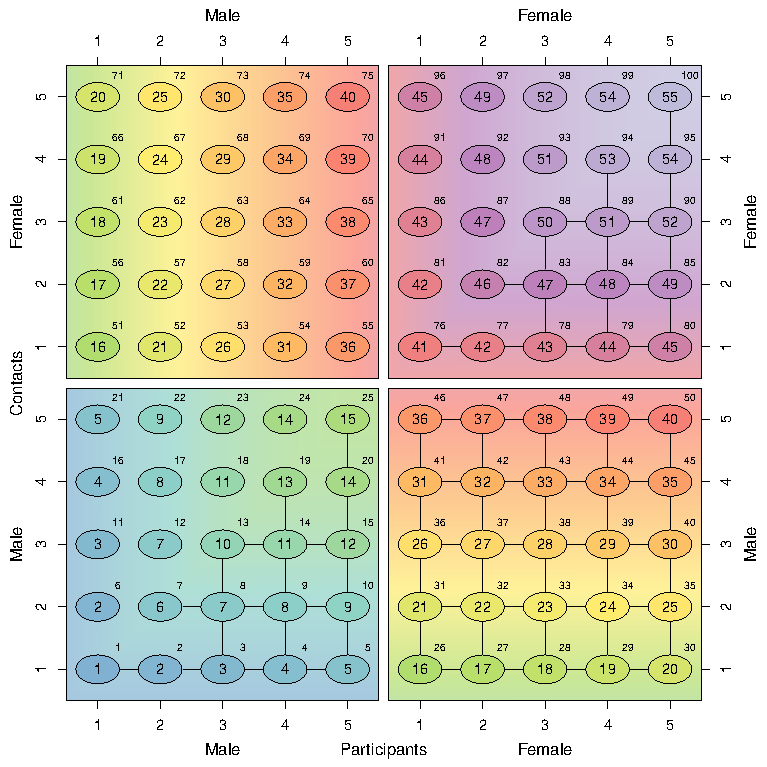
\includegraphics{fig_contact_matrix_construct.pdf}
\caption{Graphical representation of the construction of a smooth and symmetric contact matrix stratified by age ($n = 5$ age groups) and sex. Contacts are categorized as male-to-male (bottom left panel), female-to-male (bottom right panel), male-to-female (top left panel), and female-to-female (top right panel). The horizontal axis of each panel gives the age of the participants; the vertical axis gives the age of the contacts. The data records, indicated by superscripts, are numbered sequentially 1 to 100. The nodes, indicated by ellipses, are numbered sequentially 1 to 55 and ordered such that symmetry between ages and sexes is guaranteed. For illustrative purpose, identical nodes are indicated by identical colors. The edges denote the dependencies between triplets of nodes (RW2 prior).} \label{fig:1}
\end{figure}

A tailor-made construction of the precision matrix $\bm{Q}$ of the GMRF prior allows us to impose smoothness in contact rates while simultaneously accounting for the reciprocity of contacts. It is essential that the contact rates are symmetric, such that $c_\mathit{ij}^\mathit{MM} = c_\mathit{ji}^\mathit{MM}$, $c_\mathit{ij}^\mathit{MF} = c_\mathit{ji}^\mathit{FM}$ and $c_\mathit{ij}^\mathit{FF} = c_\mathit{ji}^\mathit{FF}$. These symmetries for $\bm{c}$ imply a symmetry in the deviations $\bm{x}$. Figure \ref{fig:1} provides a schematic illustration for two sexes and $n = 5$ age groups: the $5 \times 5 \times 4 = 100$ elements correspond to the 100 nodes in this graph; symmetry in value for each element is guaranteed by forcing identical values in the lower and upper triangular parts of the matrix. For example, data records 2 and 6 provide information for node 2. Thus, 55 unique node values are inferred from the 100 data records.

Smoothing is achieved by imposing the condition that neighboring node values of $\bm{x}$ should be similar. The neighborhood structure is defined by the entries of the structure matrix. Figure \ref{fig:1} provides a schematic illustration: the non-zero elements of structure matrix $\bm{R}$ correspond to the edges in this graph. Only the nodes in the lower triangular part of the matrix need to be linked, the values for the nodes in the upper triangular part follow directly because of the imposed symmetry.

We use the second order random walk prior (RW2) \citep{rue_gaussian_2005}, which reflects the prior belief that the gradient of $\bm{x}$ varies smoothly and that sudden jumps between neighboring values of the gradient are unlikely, in other words, regularize the difference of the differences. Other options include the RW1 prior, which reflects the prior belief that sudden jumps between neighboring values are unlikely, or higher order RW priors. For the RW2 prior in one dimension a Normal prior is put on the second order differences:
\begin{equation}\label{eq:2.10}
\Delta^2 x_i = x_{i-1}-2x_i+x_{i+1} \sim \text{Normal}(0, \tau).
\end{equation}
Let us for the moment consider the \textit{FM} contacts with $n = 5$ age groups, as in the lower right panel of Figure \ref{fig:1}. Here $\bm{x}^\textit{FM}$ is a $5 \times 5$ matrix. In two dimensions, smoothness is achieved by placing the RW2 prior on the rows and columns of $\bm{x}^\textit{FM}$ simultaneously. We follow the approach by \cite{currie_smoothing_2004}, using Kronecker products to construct a two-dimensional prior.

Let $\bm{D}_0$ be the matrix form of the one-dimensional difference operator in equation \ref{eq:2.10}. For $n = 5$ it has size $3 \times 5$, because near the two boundaries it is impossible to take second order differences. The difference operator matrix operating on all rows and columns of $\bm{x}^\textit{FM}$ simultaneously can then be written as $[\bm{D}_1 : \bm{D}_2]^\textit{FM}$, with
\begin{equation}\label{eq:2.11}
\bm{D}_1 = \bm{I}_n \otimes \bm{D}_0 \; \text{and} \; \bm{D}_2 = \bm{D}_0 \otimes \bm{I}_n.
\end{equation}
$\bm{D}_1$ operates in horizontal direction along the age of the participants, while $\bm{D}_2$ operates in vertical direction along the age of the contacts. Both $\bm{D}_1$ and $\bm{D}_2$ have size $15 \times 25$, so $[\bm{D}_1 : \bm{D}_2]^\textit{FM}$ has size $30 \times 25$ and operates on $\text{vec}(\bm{x}^\textit{FM}) = (x_{1,1}^\textit{FM}, x_{2,1}^\textit{FM}, \dots, x_{5,5}^\textit{FM})$ of length 25.

Next, we consider the \textit{MM} contacts with $n = 5$ age groups, as in the lower left panel of Figure \ref{fig:1}. Using equation \ref{eq:2.11}, we can construct a similar difference operator matrix $[\bm{D}_1 : \bm{D}_2]^\textit{MM}$ for $\text{vec}(\bm{x}^\textit{MM})$. However, because of the imposed symmetry, we only need to estimate the lower triangular part (including the diagonal), so $\text{vec}(\bm{x}^\textit{MM})$ is a vector of length 15. As it is impossible to take second order differences near the boundaries of the triangle (the missing edges between nodes 2 and 6, and 13 and 14 in Figure \ref{fig:1}), we can subsequently drop the corresponding rows and columns of $[\bm{D}_1 : \bm{D}_2]^\textit{MM}$, which then reduces to a $12 \times 15$ matrix. The same applies to the \textit{FF} contacts. No difference operator matrix is needed for the \textit{MF} contacts because of the imposed symmetry.

The three resulting difference operator matrices are put together in one block diagonal difference operator matrix $\bm{D}$ of size $54 \times 55$. This matrix operates on all 55 elements in $\bm{x}$ simultaneously. The corresponding $55 \times 55$ structure matrix $\bm{R}$ of the GMRF is given by $\bm{D}^\text{T}\bm{D}$ \citep{rue_gaussian_2005}. The resulting prior is improper because the precision matrix $\bm{Q}$ is not of full rank (rank deficiency is $3 \times 2 \times 2 = 12$). The posterior, however, is proper. A similar principle applies to $n$ age groups and other RW priors. The implementation can be found in the \ref{SM}.

\subsection{Model choice and validation}

We examine the effect of applying RW1, RW2 and RW3 priors. The models are compared in terms of the Watanabe-Akaike or widely applicable information criterion (WAIC) \citep{watanabe_widely_2013}. We compute the probability integral transform (PIT) to check the validity of the models \citep{dawid_present_1984}. The sensitivity of the outcome to the particular choice of hyper priors is examined using the methodology described in \cite{roos_sensitivity_2015}.

The WAIC closely approximates Bayesian cross-validation and can be viewed as an improvement on the deviance information criterion (DIC) for Bayesian models \citep{gelman_understanding_2014}. The PIT can be used as a Bayesian 'leave-one-out' predictive measure of fit or calibration check. If the observation is drawn from the predictive distribution, the PIT has a standard uniform distribution. The PIT is usually being visualized in histograms. We use the nonrandomized version of the PIT that is suitable for count data \citep{czado_predictive_2009}. The sensitivity to the hyper priors is examined by comparing the local change in the posterior parameter distribution to the unmodified posterior, in case the prior distribution is modified in a standardized way. This can be done without rerunning the model \citep{roos_sensitivity_2015}. The sensitivity is summarized by a single number, here the worst-case sensitivity, expressed as a percentage. Percentages above 100\% indicate super-sensitivity.

\section{Application}

\subsection{Contact survey data}

We use data from a prospective survey of social contact patterns to illustrate our method. Data were collected within the POLYMOD multi-country study. The goal of this study was to quantify contact behavior relevant for the spread of infections by the respiratory or close-contact route. A detailed description of the study design has been provided in \cite{mossong_social_2008}. Because of differences in data collection between countries, we only use data from the Netherlands, in which 825 participants recorded characteristics of 11,225 contacts with unique individuals during one day. As the multi-country dataset was published while data collection was still going on in the Netherlands, only 269 of these 825 Dutch participants were included in the study published by \cite{mossong_social_2008}. The additional 556 participants have been included in our analysis. Data collection took place in 2006 and 2007.

Participants were asked to complete a diary on one assigned day on the individuals with whom they had contact, as defined in section 2.1. Participants were asked to record their own age and sex, as well as the age and sex of each contacted person. There were three different types of diaries: one for children (age 0 - 8), which was completed by their parents; one for teens (age 9 - 17); and one for adults (age 18+).

Some participants reported the age of contacts as a range. We multiple imputed (10 times) these records by uniformly sampling an age from that range. From age 20 onwards, the reported age of contacts showed a preference at ages that were multiples of five. To prevent spurious results, we corrected these ages by uniformly redistributing the peak in an age range between two years younger and two years older. The additional uncertainty associated with the multiple imputations are included in all results.

Because only 22 participants reported the maximum number of contacts of 45, we ignored possible right censoring of the number of contacts. We only analyzed the reported contacts and ignored the missed contacts (see \ref{SM}). Four participants reported not having any contacts. We excluded records where there was no information on the age or sex of participants or contacts. We also excluded contacts older than 80 years, because only individuals of age 0 - 80 participated in the contact survey. For these reasons, in total 53 participants and 1,037 contacts were excluded.

The total observed number of contacts of any age and sex-specific combination, $y_\mathit{ij}^\mathit{MM}$, $y_\mathit{ij}^\mathit{FM}$, $y_\mathit{ij}^\mathit{MF}$ and $y_\mathit{ij}^\mathit{FF}$, is found by cross tabulation of the participant ID's in the data set, stratified by participant age, contact age, participant sex and contact sex. The total number of participants of any age and sex-specific combination, $t_i^M$ and $t_i^F$, is found by tabulation of the number of unique participant ID’s, stratified by participant age and sex. The age and sex-specific population numbers $w_j^M$ and $w_j^F$ with reference date January 1, 2007, are obtained from Statistics Netherlands \citep{statline_population_2015}.

The three observables $\bm{y}$, $\bm{t}$ and $\bm{w}$ are assembled into one large dataset. For each record the denominator $U_\mathit{ij}$ is calculated. The value of the denominator, which is typically $\mathcal{O}(10^6)$, is scaled by dividing the value by one million contacts. If there are no participants of age $i$, the number of contacts $y_\mathit{ij}$ is set to a missing value and the value of $U_\mathit{ij}$ is set to 1. In that way, these records do not contribute to the likelihood in the estimation procedure. Details are found in the \ref{SM}.

\subsection{Crude and smoothed contact rates}

The crude age and sex-specific contact rates $\bm{c}$ are shown in Figure \ref{fig:2}. With "crude" we mean contact rates that are directy calculated from the data without applying any regularization. They are obtained by equation \ref{eq:2.3}, where $\text{E}(\bm{Y})$ is replaced by $\bm{y}$. There are no male participants of age 25 and 80, and no female participants of age 80, resulting in white vertical lines (not visible at age 80). The values of the crude contact rates fluctuate, are often equal to zero and are not necessarily symmetric.

\begin{figure}
\centering
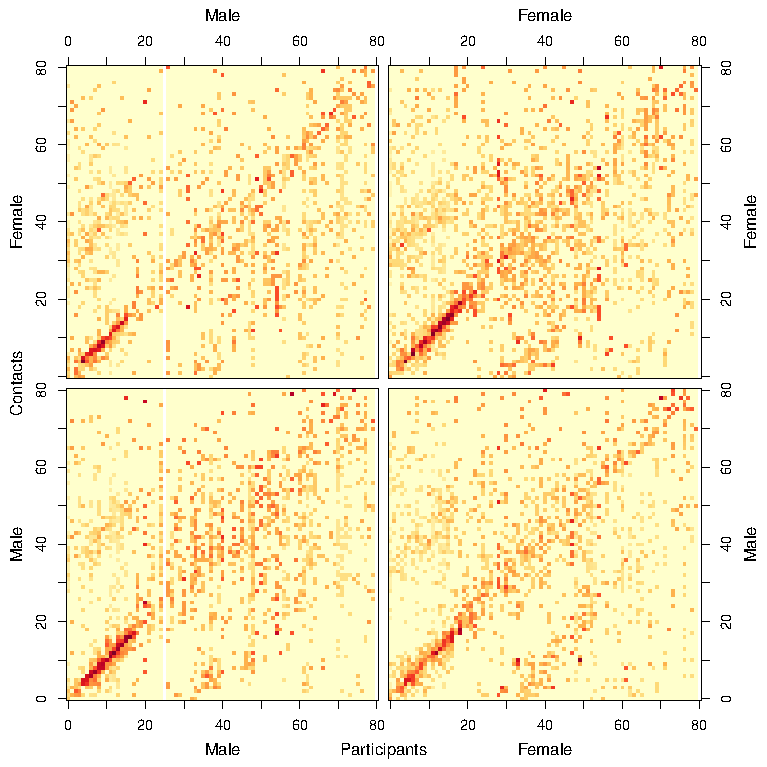
\includegraphics{fig_contact_matrix_crude.pdf}
\caption{Crude age and sex-specific contact rates. Similar to Figure \ref{fig:1}, contacts are categorized as male-to-male (bottom left panel), female-to-male (bottom right panel), male-to-female (top left panel), and female-to-female (top right panel). The horizontal axis of each panel gives the age of the participants; the vertical axis gives the age of the contacts. The color scale indicates the relative values of the contact rates from low (yellow) to high (red).} \label{fig:2}
\end{figure}

\begin{figure}
\centering
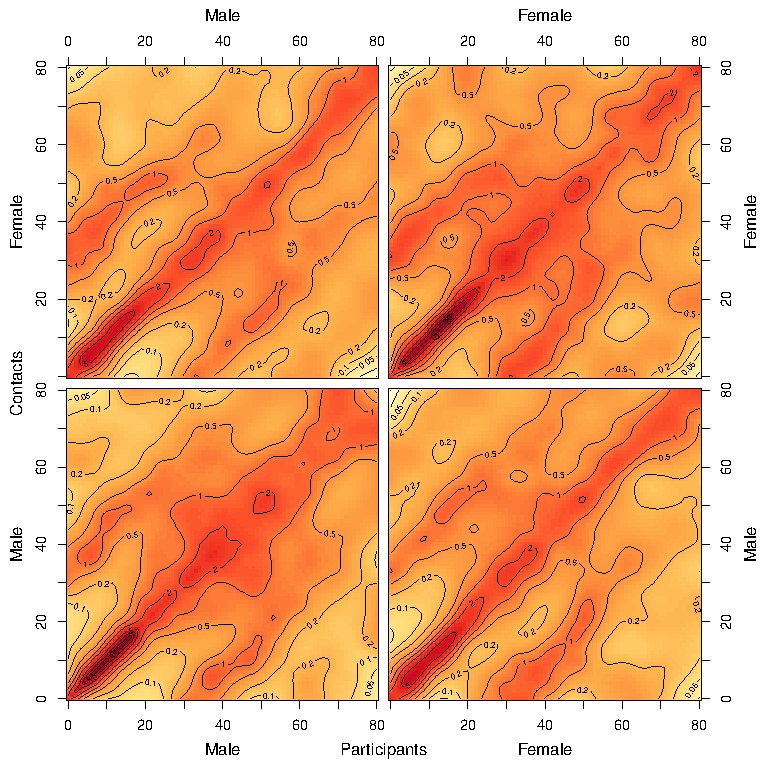
\includegraphics{fig_contact_matrix_smooth.pdf}
\caption{Estimated smooth and symmetric age and sex-specific contact rates. The color scale indicates the relative values of the contact rates from low (yellow) to high (red); the contour lines are the absolute values of the contact rates per $10^6$.}
\label{fig:3}
\end{figure}

\begin{figure}
\centering
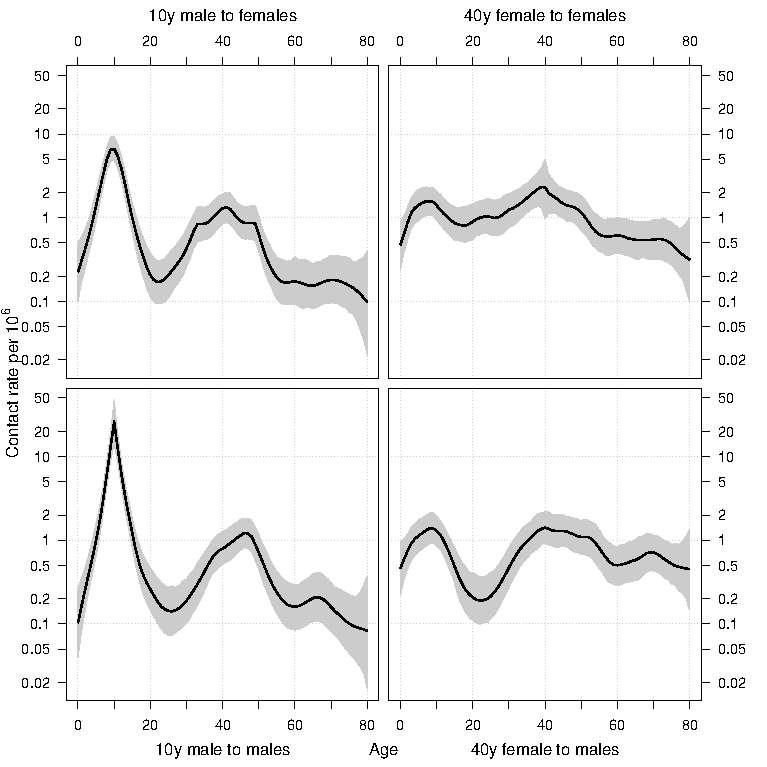
\includegraphics{fig_cross_section.pdf}
\caption{Cross-sections of Figure \ref{fig:3} showing the contact rates per $10^6$ for a male participant at age 10 having contact with males (bottom left panel) and females (top left panel), and a female participant at age 40 having contact with males (bottom right panel) and females (top right panel). Shaded areas indicate 95\% credible intervals.}
\label{fig:4}
\end{figure}

Figure \ref{fig:3} shows the age and sex-specific contact rates after smoothing while accounting for reciprocity, using the approach as described in section 2, using the RW2 prior. Reciprocity of contact imposes symmetry on the four panels, with the axis of symmetry running diagonal from the bottom left to the top right. The figure reveals highly structured contact rates that strongly depend on age. Higher rates occur along the diagonals. This indicates that contacts are mostly assortative with respect to age: people contact other people of their own age. Children and adolescents have the highest rates. The assortative pattern with respect to age continues in adults, although contacts rates become lower and more diffuse with respect to age. For children and adolescents, contacts are also assortative with respect to sex: children and adolescents contact other children and adolescents of their own sex. For adults the assortative pattern with respect to sex disappears: adults contact other adults regardless of their sex. Disassortative patterns are also present. Children have more contact with adults who are approximately 30 years older than with adults. Women have higher contact rates with children than men.

Figure \ref{fig:4} shows cross-sections of Figure \ref{fig:3} for a male participant at age 10 and a female participant at age 40. The figure illustrates the uncertainties associated with the estimates. Contact rates for a 10 year old male with other males and females of different ages increase rapidly with age, having a sharp maximum with 10 year old males and females (classmates) and reaching another peak with 45 year old males (fathers) and 40 year old females (mothers). Contact rates for a 40 year old female with other males and females of different ages show a more gradual pattern. Note the discontinuity in the gradient at contact age 10 (10 year old males) and contact age 40 (40 year old females) as a result of the tailor made prior distribution.

\subsection{Model choice and validation}

Table \ref{tab:1} shows the WAIC and effective number of parameters for models with three different RW priors. The RW2 prior resulted in the lowest WAIC, and is therefore to be preferred. The RW1 prior implies the least regularization and highest effective number of parameters, the RW3 prior implies the most regularization, the smoothest surface and lowest effective number of parameters.

Figure \ref{fig:5} shows the PIT histograms for three models with different RW priors. In particular the histograms for the models with RW2 and RW3 prior are nearly uniform, indicating a good model fit, i.e. the observations are drawn from the predictive distribution.

The worst-case sensitivity estimates of the hyper parameters were 13\% for the log-transformed precision parameter $\tau$ and 0.25\% for the log-transformed dispersion parameter $\theta$. These values indicate that the posterior distributions for the contact intensities are insensitive to the choice of the prior parameter values.

\begin{table}
\caption{Comparison of three different priors for smoothing the contact rates, with the widely applicable information criterion $WAIC$ and effective number of parameters $p_{eff}$. The lowest value of the $WAIC$ indicates the most parsimonious model.}
\begin{tabular}{l r r}
\hline
Prior & $WAIC$ & $p_{eff}$ \\
\hline
RW1 & 32505.5 & 1620.0 \\
RW2 & \underline{32431.3} & 479.3 \\
RW3 & 32660.0 & 261.6 \\
\hline
\end{tabular}
\label{tab:1}
\end{table}

\begin{figure}
\centering
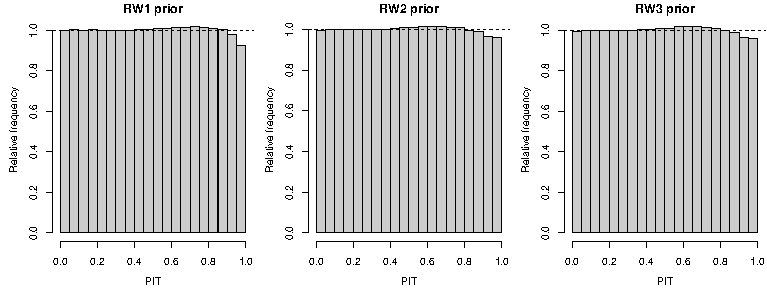
\includegraphics{fig_pit.pdf}
\caption{PIT histograms for three models with different RW priors. The histograms show the probability integral transform of the observed total number of contacts relative to the model predictions.} \label{fig:5}
\end{figure}

\subsection{Differences in projected age-specific risk of infection between the sexes}

The estimated contact rates could result in relevant differences between the sexes with respect to the age-specific risk of acquiring respiratory infections. To explore whether such differences occur, the posterior contact rates are converted into contact intensities by applying equation \ref{eq:2.3}, e.g. for male-to-female contacts $m_\textit{ij}^\textit{MF} = c_\textit{ij}^\textit{MF} w_j^F$, and assemble contact intensities into a block matrix. This matrix is called the next generation matrix. In our notation of this matrix, the index $i$ refers to the characteristics of the infectors and the index $j$ to the characteristics of the infected. The right dominant eigenvector of this matrix can be interpreted as the age and sex-specific risk of an infection that is transmitted via close contacts or respiratory droplets when a new emerging infection spreads in a completely susceptible population \citep{wallinga_optimizing_2010}. Here we use this right dominant eigenvector to quantify possible differences between the sexes to the age-specific risk of infection.

The resulting normalized age-specific risk of infection shows differences between the sexes (Figure \ref{fig:6}a). The infection risk increases at a young age, from a relatively low risk for infants to a high risk for teenagers. There is a sharp decrease in infection risk for young adults, followed a modest rise in risk around the age of 40. For older ages the risk decreases again. The ratio between infection risk of females and males shows that between ages 18 - 38 women have a significantly higher infection risk than men, and between ages 50 - 65 women have a lower risk than men (Figure \ref{fig:6}b).

\begin{figure}
\centering
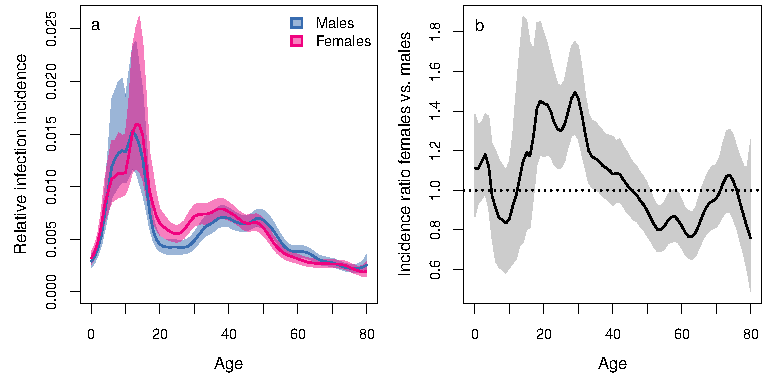
\includegraphics{fig_relative_infection_incidence.pdf}
\caption{Projected risk of infection, based on the estimated contact rates. a) Relative incidence of infection when a new emerging infection spreads in a completely susceptible population. b) Incidence ratio between females and males; above the dotted horizontal line females have higher incidence compared to males. Shaded areas indicate 95\% credible intervals.} \label{fig:6}
\end{figure}

\begin{figure}
\centering
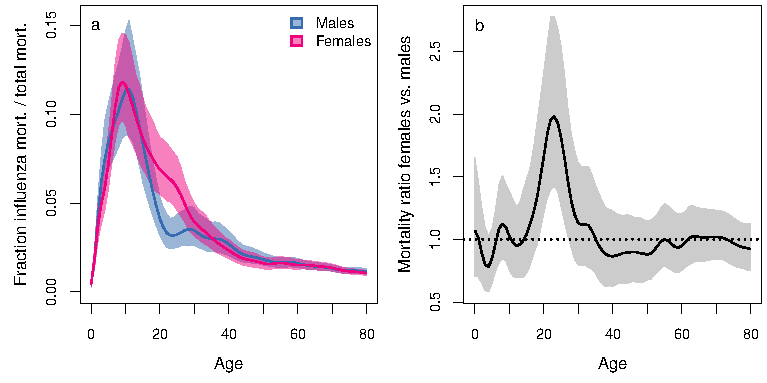
\includegraphics{fig_influenza_mortality.pdf}
\caption{Observed risk of death upon infection during the 1957 influenza pandemic in the Netherlands. a) Risk of death due to influenza relative to all-cause mortality by age and sex. b) Mortality ratio between females and males.} \label{fig:7}
\end{figure}

We compared these contrasting age-specific infection risks for men and women to observations on influenza related mortality during the 1957 influenza pandemic in the Netherlands. We calculated the age and sex-specific fraction of deaths due to the 1957 influenza pandemic relative to total number of deaths in the Netherlands \citep{polak_influenzasterfte_1959}. Mortality rates were modeled by a Poisson generalized additive model using penalized splines for age. The mortality rates increase at a young age, from low rates for infants to high rates for teenagers. The broad pattern is similar to that of the projected infection risk: there is a decrease in infection risk for young adults, followed by a leveling off at the age of 40. For older ages the risk decreases further (Figure \ref{fig:7}a). The ratio between mortality rates of females and males shows that between the ages 20 - 30 women have a significantly higher risk than men (Figure \ref{fig:7}b). Figure \ref{fig:6} compared to Figure \ref{fig:7} shows that the differences in infection risk between the sexes, as expected from the observed age and sex-specific social contact patterns, could account to a large extend for the differences in mortality risk due to infection, as observed in mortality statistics.

\section{Discussion and conclusions}

We have estimated social contact rates at an unprecedented level of detail for men and women of all ages. The estimation of contact rates requires smoothing while at the same time enforcing consistency with reciprocal nature of contacts. We achieve smoothing by a Gaussian Markov Random Field approach where we impose a random walk prior in two dimensions directly on the logarithm of the age-specific contact rates. 

The proposed approach has important advantages over existing alternatives. First, the proposed approach makes it possible to increase the resolution up to 81-year age cohorts and stratification by sex. This is a significant improvement over existing methods for statistical analysis of social contact data that aggregate the entire age range in six crude age classes \citep{wallinga_using_2006} or 16 age classes \citep{mossong_social_2008}, and ignore sex. Second, we are able to explicitly specify the reciprocity constraints. This is a significant improvement over existing methods that do not guarantee reciprocity and risk inconsistent outcomes \citep{mossong_social_2008}. Third, the amount of smoothing is directly estimated from the amount of information in the data, and we can specify where the borders of smooth surfaces are located - at the boundaries and along the diagonal of the contact matrix - therefore preventing undesired artifacts such as smoothing across the diagonal. This is a significant improvement over existing methods that use a smoothing tensor spline with constraints \citep{goeyvaerts_estimating_2010}. Fourth, the proposed approach allows for fast and efficient estimation of contact rates. One model run takes a few minutes on a standard desktop computer.

The estimated social contact patterns require a critical checking with respect to model choice, validity and prior sensitivity. The patterns also require a critical checking with respect to plausibility to patterns of disease transmission. We will briefly look at each of these aspects in turn.

We have described the total number of contacts by a Negative Binomial distribution that is parameterized with a mean and a dispersion parameter. The mean is allowed to vary by age and sex. In this study we focus on the expected contact rates and therefore we treat the dispersion parameter $\theta$ and precision or smoothing parameter $\tau$ as nuisance parameters. If these parameters would be of direct interest they can be varied by age and sex, although this would be computationally challenging. We believe that it is a reasonable assumption that the dispersion and rate of change between ages for the contact process between men, between men and women, and between women are the same for all sexes.

Based on the WAIC, the RW2 prior is the preferred prior. In frequentist statistics it is common use to penalize the second derivative of the curve \citep{wood_generalized_2006}. Particularly in P-spline smoothing it is a common use to put a discrete second order penalty on the spline coefficients \citep{eilers_flexible_1996}. In a Bayesian context, this is exactly the same as putting a RW2 prior on the coefficients \citep{lang_bayesian_2004}. Our 2-dimensional RW2 prior is based on the work by \cite{currie_smoothing_2004}, where second order differences in both the horizontal and vertical dimension are taken simultaneously. Our approach is a simple and intuitive way of constructing a smoother in two dimensions for triangular shaped grids. To develop some intuition for the proposed 2-dimensional RW2 prior: simulated realizations for a specified marginal prior variance and prior correlations for $n = 81$ and a fixed $\tau$ reveal that the prior variance is the largest near the boundaries and along the diagonal of the grid and that prior variance decreases towards the interior parts. The prior correlation between some given node and its surrounding nodes decreases with node distance. There are alternative approaches possible for a prior. A 2-dimensional RW2 prior could be constructed by applying the biharmonic operator, a discrete analogue of thin plate splines \citep{rue_gaussian_2005}. Adapting this prior to a triangular grid as required here is challenging.

The validity of the model was checked using PIT histograms \citep{czado_predictive_2009}. The model accurately reflects the contact data as reported by the survey participants. We have examined prior sensitivity using the methodology described in \cite{roos_sensitivity_2015}. The results indicated that the posterior distributions are insensitive to the choice of the prior hyper parameter values.

We checked the relevance of the estimated contact intensities as proxy measure for transmission of infection by comparing the project risk of infection to actual risk of mortality upon infection with influenza during the 1957 influenza pandemic. We chose the 1957 pandemic as it was the last large epidemic of a respiratory infection that hit an almost completely susceptible population in the Netherlands, and therefore provided the closest comparison with the model projections. As we cannot rule out any differences in age-dependent mortality rates between the sexes, and as the study population for the contact survey was not representative for the general population in 1957, this test does suggest that the estimated age- and sex-specific contact intensities sexes could provide a parsimonious explanation for much of the observed difference in mortality between the sexes. This contrasts with an implicit, but dominating assumption in the study of infectious diseases, that risk of respiratory infection is determined by age, and that sex-differences in risk of infection are negligible \citep{klein_impact_2010}. Our findings suggest that, within each age group, much of the observed variation risk of infection within age groups might be due to sex-specific differences.

Additionally, we checked whether the findings can be repeated with similar data sets, for instance contact data collected in several different European countries in the POLYMOD study \citep{mossong_social_2008}, and with these data stratified even further by day of the week and by contact setting (home, school, work, leisure, transport and other). We found a very similar overall contact patterns with respect to age and sex. Even though this additional analysis has some inconsistencies because the reciprocity of contacts, which holds true by definition over all settings, may become questionable for contacts within settings, its outcome strongly suggests that the estimated patterns are very plausible, and not specific to the particular contact data we have used here.

The observed differences in the contact pattern of adult men and women indicate that sex differences in infection risk only come into play when there is significant risk of infection for adults. This is the case for vaccine-preventable diseases where a high vaccination coverage increased the age at infection, such as measles, mumps, and rubella; for diseases that are poorly transmissible, such as human parvovirus B19 \citep{young_parvovirus_2004}, and diseases that cause repeated infections, such as influenza A, B \citep{klein_impact_2010} and cytomegalovirus \citep{pass_vaccine_2009}. Furthermore, detailed social contact patterns help to improve the parameterization of mathematical models used to design and evaluate control strategies, allowing for models that are more realistic. In particular, the highly detailed age-specific contacts are relevant for evaluating vaccination schedules aimed at protecting infants against diseases such as pertussis or pneumococcal infections and sex-specific contacts are relevant for evaluating vaccination schedules aimed to protect against infections that complicate pregnancy or may lead to spontaneous abortion, such as rubella virus, human parvovirus B19, or cytomegalovirus.

Social contact intensities between men and women of all ages can be estimated using hierarchical Bayesian modeling approach with an underlying Gaussian Markov Random Field. A tailor-made construction of the precision matrix of the GMRF prior allows us to regularize the estimates by smoothing while at the same time enforces consistency with reciprocal nature of contacts. Estimation can be done efficiently using Integrated Nested Laplace Approximations. Application of this approach to social contact data from a large prospective survey revealed that social contact patterns, as a rule, are assortative: people, especially children and adolescents, mostly contact other people of their own age and sex. Relevant exceptions are that children have more contact with adults who are approximately 30 years older than with other adults, and women have more contact with children than men. These social contact patterns result in exposure patterns that significantly differ between sexes. For an emerging respiratory infection that spreads in a susceptible population, we would expect the risk of infection to vary for three broad age categories: for children, the risk of infection is similarly high for both sexes; for younger adults, women are at higher risk of infection; for older adults, men are at higher risk of infection.

\section*{Acknowledgements}
The authors thank Janneke Heijne for providing the contact data from the POLYMOD study in the Netherlands, and H\r{a}rvard Rue and Albert Wong for their useful suggestions concerning the construction of the structure matrix. Special thanks to all reviewers and editors who have provided critical and constructive comments that have helped to improve the manuscript considerably.

% Supplement
\begin{supplement}
\sname{Supplementary material}\label{SM}
\stitle{Efficient estimation of age-specific social contact rates between men and women}
\slink[url]{link will follow in final version}
\end{supplement}

% References
\bibliographystyle{imsart-nameyear}
\bibliography{Contact_Patterns}

\end{document}
